\section{Introduction}
\subsection{Problématique}
La problématique de la stabilisation tonale est une problématique qui a été peu étudiée. En effet, les appareils personnels de prise de vue se sont démocratisés il y a peu de temps, et l'introduction dans ces appareils de système de balance de couleur et de changement d'exposition automatique fait que ce problème est très récent. La figure \ref{fig_unstable} montre deux images à moins d'une seconde d'intervalle. On peut remarquer une variation importante de la tonalité de l'image alors que la scène a très peu changé.\\

\begin{figure}[H]
\centering
\begin{tabular}{cc}
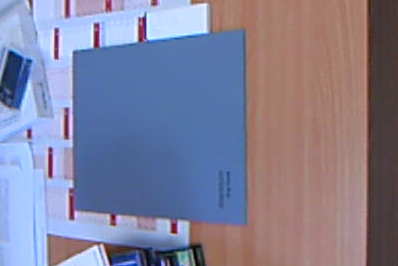
\includegraphics[width=0.4\textwidth]{Chapters/Images/fig_unstable2}&
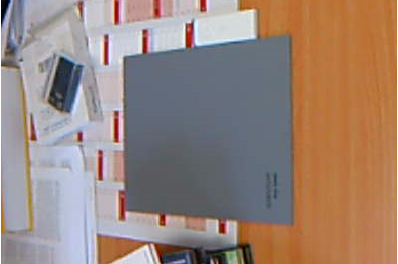
\includegraphics[width=0.4\textwidth]{Chapters/Images/fig_unstable22}
\end{tabular}
\caption{Instabilité tonale}
\label{fig_unstable}
\end{figure}

Dans les appareils personnels, des ajustements temps réel de l'exposition des vidéos et de balance des blancs sont fait et, d'après les auteurs de l'article, désactiver l'automatisation de ces réglages d'exposition ne peut être une solution à cause de la dynamique des scènes qui peut être très variable notamment. \\

La récente démocratisation de ces caméras, et des moyens de diffusion de vidéos, apporte un intérêt certain à la problématique de la correction de ces fluctuation tonales. Cependant, chaque appareil peut avoir ses propres algorithmes de corrections, et les paramètres tonaux de ces caméras varient aussi. Ainsi, les auteurs de l'article ne veulent pas introduire dans leur solution un modèle avec un fort a priori.\\

\subsection{Motivations et travaux connexes}
Les auteurs souhaitent donc réaliser un algorithme (semi) automatique de correction de ces fluctuations tonales. Les auteurs notent que l'on pourrait utiliser des méthodes permettant de modéliser la réponse tonale des caméras afin de l'inverser, cependant les méthodes existantes nécessitent d'utiliser des images recalées pour lesquelles la seule variation est l'exposition.\\

Un second type de méthode qui pourrait être utilisé consiste à effectuer un transfert de couleur global entre une image ancre et l'image que l'on souhaite stabiliser. Cependant, les mouvements de la caméra et les objets de la scène perturbent les statistiques de l'image, et rendent  donc ces méthodes peu efficaces. Les méthodes locales de transfert de couleur, elles, sont soumise à la problématique de la mise en correspondance de zone dans l'image, problème non trivial.\\

